\chapter{Background studies} \label{stateofarts}
Before beginning with the design and development of the prototype application, a fundamental base of knowledge has to be set. This chapter gives definitions about the most important terms and concepts used in VR. The context in which this project is set in is also explained briefly. Furthermore, this chapter specifies the most important technologies for the prototype and also points out where the limits of VR are. Finally, a measurement for the effectiveness of  VR is presented.

\section{Context}
The prototype application will be focused on the information technology diploma courses offered at the Nanyang Polytechnic. In the following, the environment of the school and the courses will be described.

Nanyang Polytechnic (NYP) is a polytechnic located in Ang Mo Kio, Singapore. The school offers post-secondary education for students who successfully passed the GCE O-Level examination. The O-Level examination is an annually examination mainly for students who have visited a secondary school. \cite{aboutOLevel} \\ 
This examination allows students to take courses either on a junior college, a technical institute or a polytechnic. In Singapore, a polytechnic offers students a more practical and industry based education than a junior college, which has a more theoretical approach. In general, students study 3 years at a polytechnic until they get their diploma. After getting a diploma, students can continue their education at a university but they can also start to work in the industry. \cite{schoolSystem}
\subsection{NYP information technology courses}
NYP offers a wide range of courses in different fields. One of the fields is information technology (IT). In the following the courses will be introduced briefly: \cite{nypCourses}

\paragraph{Information Technology}
This course offers students a broad range of different fields in information technology. It focuses on an interdisciplinary education. By finishing the course, students are prepared to work in different areas, most commonly in software engineering. During the first year, the fundamental topics of information technology are educated. The second year deepens the knowledge in application programming, database management, software engineering, algorithms and several other topics. The third year will be for specialization. The students can choose between elective courses in the fields of artificial intelligence, enterprise cloud computing, geospatial and mobile innovation and cybersecurity. As in all courses offered at the school of information technology, there is offered one practical industry project and an internship in the third year as well.

\paragraph{Infocomm and Security}
This course covers topics in IT infrastructure, network engineering and security and the internet of things (IoT). Students learn how to program, but also how to secure applications in a connected environment and they learn about managing connected infrastructures. During the first year there are basic classes in programming and infocomm to get a grounded knowledge in information technology. The second year will deepen the knowledge of network engineering, programming, and IT service management. There will be a practical IoT project for students as well.
In the third year there are several elective courses in the areas of system and network security, enterprise infrastructure and infocomm solutions.

\paragraph{Cybersecurity and Digital Forensics}
The cybersecurity and digital forensic course focuses on IT security. This includes securing systems and data for unauthorized access as well as tracing criminals in case of a security incident. After graduating, students can work as security analysts, network penetration tester, security engineer and similar positions. During the first year students learn fundamental IT skills. The second year offers classes in forensics, network security, operating systems, security standards and more. Students will also complete an applications security and an infosecurity project.
The last year offers specialization in the topics cybersecurity track and cyber forensics track. It is possible to choose crossdisciplinary classes from other IT courses.

\paragraph{Business Intelligence and Analytics}
The business intelligence and analytics course teaches analytics and interpretation of massive amounts of data. Therefore big data technologies as well as artificial intelligence is needed. After graduating, it is possible to work as a data or business analyst, a social media strategist or a digital marketing executive. During the first year students will gain basic IT and business statistic knowledge. The second year offers classes in big data management, digital marketing, predictive modelling and similar topics. Students participate on a big data and a business analytics project.
During the third year, students will do a data science project and can choose between several elective classes.

\paragraph{Business and Financial Technology}
This course focuses on information technology in the financial and business sector. After getting a diploma, students can work as IT or financial consultants, financial application specialists or business and financial analysts. From the beginning the focus lies on connecting business and financial topics with information technology. Therefore, in the first year students learn about economics, accounting and consumer banking as well as about basic programming skills. During the second year this knowledge is deepened through classes like software engineering or financial management. Besides the elective classes, the industry project and internship, students in their third year also collaborate in a fintech innovation project.
\section{What is virtual reality?}
\todo{Definition; use; popularity; difference from AR}
According to \cite{Fuchs.2011} VR is a simulated virtual world, created with hardware and software. It provides a real time user interaction and users feel the maximum amount of immersion when experiencing the computer generated world. The virtual world is mostly provided by a head mounted display (HMD) as seen in figure \ref{fig:hmd}. This device splits the main scene into two different camera perspectives for each eye of the user. The two perspectives will then be merged into three dimensional picture by the users brain. \\
\begin{figure}[h!]
  \includegraphics[width=70mm]{kapitel/HMD-example.jpg}
  \centering
  \caption{Head mounted display by}
  \label{fig:hmd}
\end{figure}
% by Maurizio Pesce -  \url{https://www.flickr.com/photos/pestoverde/17136177965}, CC BY 2.0, \url{https://commons.wikimedia.org/w/index.php?curid=39894108
The computation of the virtual world can either be done on a standalone desktop PC or directly in the HMD, for example through a mobile phone which is wrapped inside the HMD.\\
Different from augmented reality (AR), VR provides a fully self-contained environment and does not interact with elements of the real world. AR on the other hand embeds virtual content into the real environments. Thereby the borders between reality and simulation become blurry. AR is a closely related technology to VR, but this thesis will focus on VR applications only.\\
The usages of VR are very versatil. \cite{Linowes.2015} describes a variety of different areas in which VR can be used: Especially the gaming industry stands out for one of the first industries to develop VR applications and hardware devices. This is because most of the modern computer games take place in a computer generated, first person, 3d environment. To achieve a higher level of realism, it seems very likely to introduce VR in the gaming branche. Lately, non-gaming VR applications are getting more and more important. Design and architecture is a branch, where VR is used to visualise prototypes in a new way to customers. In education, VR applications are used to train learners in a nearly real environment but without the cost and danger of a real life exercise. Military training or disaster management are good showcases for the usage of VR in education. Another area, in which VR is used, is tourism. Through a VR application it is possible to visit a museum without actually travelling to the place. VR can give more immerse insights of a travelling destination and yet can be an instrument of marketing for the tourist destinations.
\section{VR basic concepts}
\todo{covering some history in this chapter too? E.g. explaining the first wave of VR in the 90s}
\cite{Sherman.2019} describe five core concepts for virtual reality.  According to them, this concepts are the key elements when it comes to design a virtual reality. In the following, this concepts will be explained:
\paragraph{Participants} A participant is a user of a VR application, who is actually wearing the HMD and experiencing the virtual world. Every participant has a different perception of the application, so every experience can be seen as a unique experience. This is because the several participants differ from their cultural background, their age, their expectations and their knowledge in technology. Therefore, it is a challenge for developers of VR applications to create a virtual world which various users can identify with. The role of the participants is described as the most important role, because all the experience is happening in their imagination. Developers or creators are only capable of creating the framework around the experience.
\paragraph{Creators} Creators or developers design and implement a VR application for participants. As mentioned, the developers are not able to create the experience of the users. The core aim of their work is to develop the application, which is a collection of programming scripts, concept designs and data. The experience is created together with the participants. Later in this thesis there will be an insight in developing a VR application from a creator's perspective, whilst chapter \ref{testing} will dive into the different experiences of participants using the VR application.
\paragraph{Virtual world} In general, the term "virtual world" is defined as the content of a virtual reality application.  The virtual world is the skeleton of the virtual experience. Precisely, it is a description of the objects inside the virtual space. Everything which the user can see, hear and interact within the VR application belongs to the virtual world. How the virtual world space is designed influences the experience of a participant.

\paragraph{Immersion} Immersion in general describes how deeply users connect with a virtual world. They experience something through a medium which they would not be able to experience without it. They see actions and things through a different point of view and can connect with it in some way. The deeper a user can connect to the virtual environment and the objects inside it, the more immerse is the VR experience. In chapter \ref{immersion} the term immersion will be explained in more detail.

\paragraph{Interaction} Most of the time, interaction means manipulation of a computer generated world. However, interaction can also happen in a non artificial environment. An example for this are interactive novels, or text based computer games. In this kind of media, computer graphics are not required and yet they provide a form of user interaction. When it comes to VR, interaction also means relocating a viewport inside a virtual world. Participants can move physically in the virtual environment. Another form of interaction is the collaborative interaction. In some VR applications it is not only possible to interact with the virtual world but also to share the space with other participants and interact with them. This can happen in a virtual or physical way.
\subsection{Different dimensions of reality}
\todo{describe different states: reality, augmented reality, augmented virtuality, vr}
Besides VR, there exist other technologies, which serve the purpose to create virtual worlds for the user. They differ in the extend of intervention with the reality. \cite{Tham.2018} show a spectrum of different types of technologies and their dimension of reality. A visual representation of this spectrum is displayed in \ref{fig:spectrum}.\\
\begin{figure}[h!]
  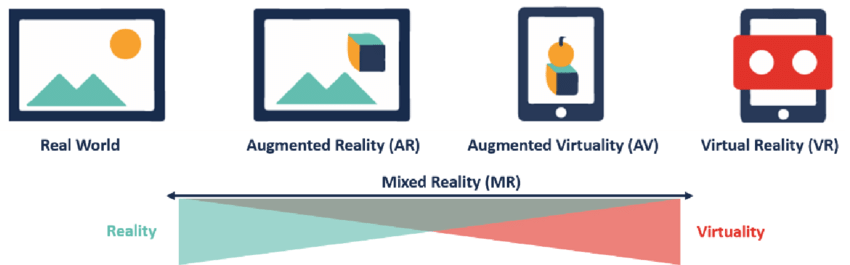
\includegraphics[width=14cm]{kapitel/spectrum-of-reality.png}
  \centering
  \caption{Graphical representation of the dimensions of reality by 	  \cite{Lovreglio.2018}}
  \label{fig:spectrum}
\end{figure}

The reality describes the real world and using non digital devices for interaction, such as a steering wheel for driving a car for example. As mentioned in the indroduction, AR is a related technology to VR. In the spectrum of \cite{Tham.2018} AR covers the second level of reality dimensions. It describes computer generated elements, which are embedded into the reality. A famous example for an AR application is the game PokemonGo (\url{https://www.pokemongo.com/en-gb/}), in which players search in the real environment for computer generated items, based on a phone's camera and location services. The next level of reality is the augmented virtuality. This term describes a virtual environment, in which users can interact through analogue methods. An example for this could be a video chat room where the participants are present in a virtual room but communicate through analogue methods. As seen in figure \ref{fig:spectrum}, augmented reality and augmented virtuality can be summed up with the term \"mixed reality\" which describes the interaction between real life elements and the virtual environment. Finally, in the last stage there is VR in which a user is fully surrounded by a computer generated environment. This environment is most likely a reproduction of a real-life environment. The user is not only surrounded by an artificial reality but can also interact with it. It might happen that the user actually feels present in the virtual reality. In the following, this phenomenon will be explained in more detail.

\subsection{Immersion and storytelling}\label{immersion}
\todo{What is immersion and why so important for VR? What describes a good storytelling? Is there anything special when designing a story for a VR application?}
The term immersion often comes up when talking about VR. This term describes an experience which users would not be able to percieve without the use of the specific medium. In general, it describes an experience from a different point of view. This could be for example the story of a different character or the exploration of a unknown location. \cite{Tham.2018} \\ Immersion is an important measurement for this work. The experience, students have when playing the VR application, which will be developed during this thesis, depends on the grade of immersion.
When talking about immersion, it is important to distinguish between  mental and physical immersion. Mental immersion describes the state, in which the participant feels deeply emotionally connected to the virtual world. Physical immersion on the other hand means that the user's physical interactions are transferred into the virtual environment with the use of technology. The movements should feel as natural as possible to the user. When talking about immersion in books, films or related media, it is often only referred to mental immersion, because these types of media are not able to provide the technology for interacting with their environments. VR on the other hand can create immersion through a physical way as well. That is why VR can provide a higher grade of immersion than other media. \cite{Tham.2018}\\
Another term closely related to immersion is presence. Presence in the context of VR describes the subjective feeling of actually existing in the virtual world. The feeling of presence is a mix between mental and physical immersion. The more presence users feel, the more they accept the virtual world as the reality. To gain the sense of presence, the participant's movements in the reality should match with the movements of the virtual world. With a higher grade of presence, participants act more natural in a virutal environment, such as they would in a real environment. Through this, their task performance increases. This is one reason why presence is an important factor when it comes to developing VR applications, especially in the field of education and learning. \cite{Slater.1997}

Since the terms immersion and presence are explained, it is now the question, how to design the story of a VR application in order to gain a maximum grade of immersion. Storytelling is one of the most important elements for mental immersion in a virtual experience. Especially mental immersion can be influenced by the storyline, while physical immersion can be increased through hardware tools. \\
Storytelling in general is the art of telling a narrative to the user in a way that the user is not only consumer but actually feels immersed with the story \cite{Louden.2018}. Designing a storyline in VR opens a lot of possibilities in engaging the participant in the story. Therefore there are things to consider when it comes to storytelling in VR as explained by \cite{Keane.2018}:\\
One thing to bear in mind is, that space and environment in a VR application are more important than in other media, like books or films. The creator designs a world in a 360 degree view, so there is a lot more space to show. The storyline not only happens in front of the users, but can be all around them. Because the user is able to walk independently in the virtual world, it is very important to softly guide users into a certain direction when necessary for the storyline. The guidance should not be conspicuous, but should attract  users' curiosity. This can be achieved through light and sound effects or movements. Another aspect to consider is not to overwhelm  users with complex tasks. This could prevent the user in experiencing an immersed virtual world because their full attention would lie on completing the tasks.
\subsection{Interaction: Selection, manipulation and navigation}
\todo{different interaction tasks in VR and their common solution: Simple virtual hand, raycasting, go-go, HOMER, scaled world-grab, occlusion; describing ways of movement (walking aroung) solutions in VR}
In order to get an immerse experience, the user of a VR application needs to interact with the environment. When it comes to interaction in VR, several challenges occur. First of all, there is a three dimensional space which has to be covered. Secondly, when users are wearing the HMDs, they cannot see the controllers they are using in the real world. This means, that every hardware controlling device should be mapped into the virtual world. This chapter describes some typical interactions and their common solutions in VR. It is a base overview of interaction methods, which can be considered to be used in the prototype VR application. The final method, which suits the best for the prototype, will be discussed in chapter \ref{design}.\\
Basically, there are two different types of interaction in VR: Modifying the virtual world and moving in the virtual world. When modifying the virtual world, the user should be able to select and manipulate objects. Manipulating includes moving, scaling, changing of look (color, texture) and orientation of an object in the virtual world. When walking around in the virtual world, the user should be able to move freely and make their own decisions in navigation. \cite{Dorner.2013}\\
A challenge when finding solutions to the described interaction problems is, that there do not exist standard solutions, like we have in a screen based 2D context for example. Nevertheless, There are some best practices on how to implement the described requirements in VR. In the following, the most common interaction techniques will be explained according to \cite{Dorner.2013}.

A very straightforward method in selection could be the selection through gaze. The user can select objects by looking at it. This is a very simple method and works without hardware controllers for user input. An analogy in 2D interfaces would be the selection via mouse over. However, this technique does not work well in VR. The problem is, that users accidentally select objects every time they look around. A simple and natural exploring of the virtual world would be interrupted by object selection.\\
Another technique is called ray-casting. It works with a virtual virtual ray coming from the users' hand. Therefore, an controller or a hand tracking hardware is needed, which movements are mapped into the virtual world. Every object which collides with the ray is a possible candidate for selection. Most of the time, the object nearest to the user will be selected. ray-casting is an important method in object selection, because it is very straightforward and conforms to the expectations of users (TODO why?). Nevertheless, this method becomes inaccurate when to deal with large distances, because the movements of the hand has to be more accurate the longer the distance gets. \\
The next method, the Go-Go technique overcomes this problem. A virtual arm, mapped with the user's hand movements is displayed in the virtual world just as done with the ray-casting method. The difference of the Go-Go- technique is, that the virtual arm can be lengthened, if the selectable object is out of range. When the virtual arm is lengthened, the user's hand movements are mapped in a smaller range, than when the virtual arm is in the normal position. This mapping is not linear and overcomes the problem of inaccuracy when selecting objects to far away. The technique can be well used for relocating objects, because the user does not have to walk on the same time. However, with this technique, as well as with the ray-casting technique, only objects which are in viewing range can be selected or manipulated. Some objects could be overlapped by other obstacles and cannot be selected. Also, objects in far distance appear very small, which makes manipulation difficult.\\
The HOMER technique deals manipulation of objects in distance. The abbreviations stands for Hand-Centered Object Manipulation Ray-casting. As the names says, it uses techniques of the ray casting for selection. To make the manipulation easier, the object moves to the users hand, once selected. The user can now perform their desired manipulation. After the manipulation is finished, the objects teleports back to its original position. This technique still has the problem of selecting objects which are not in the user's viewing range.\\
\begin{figure}[h!]
  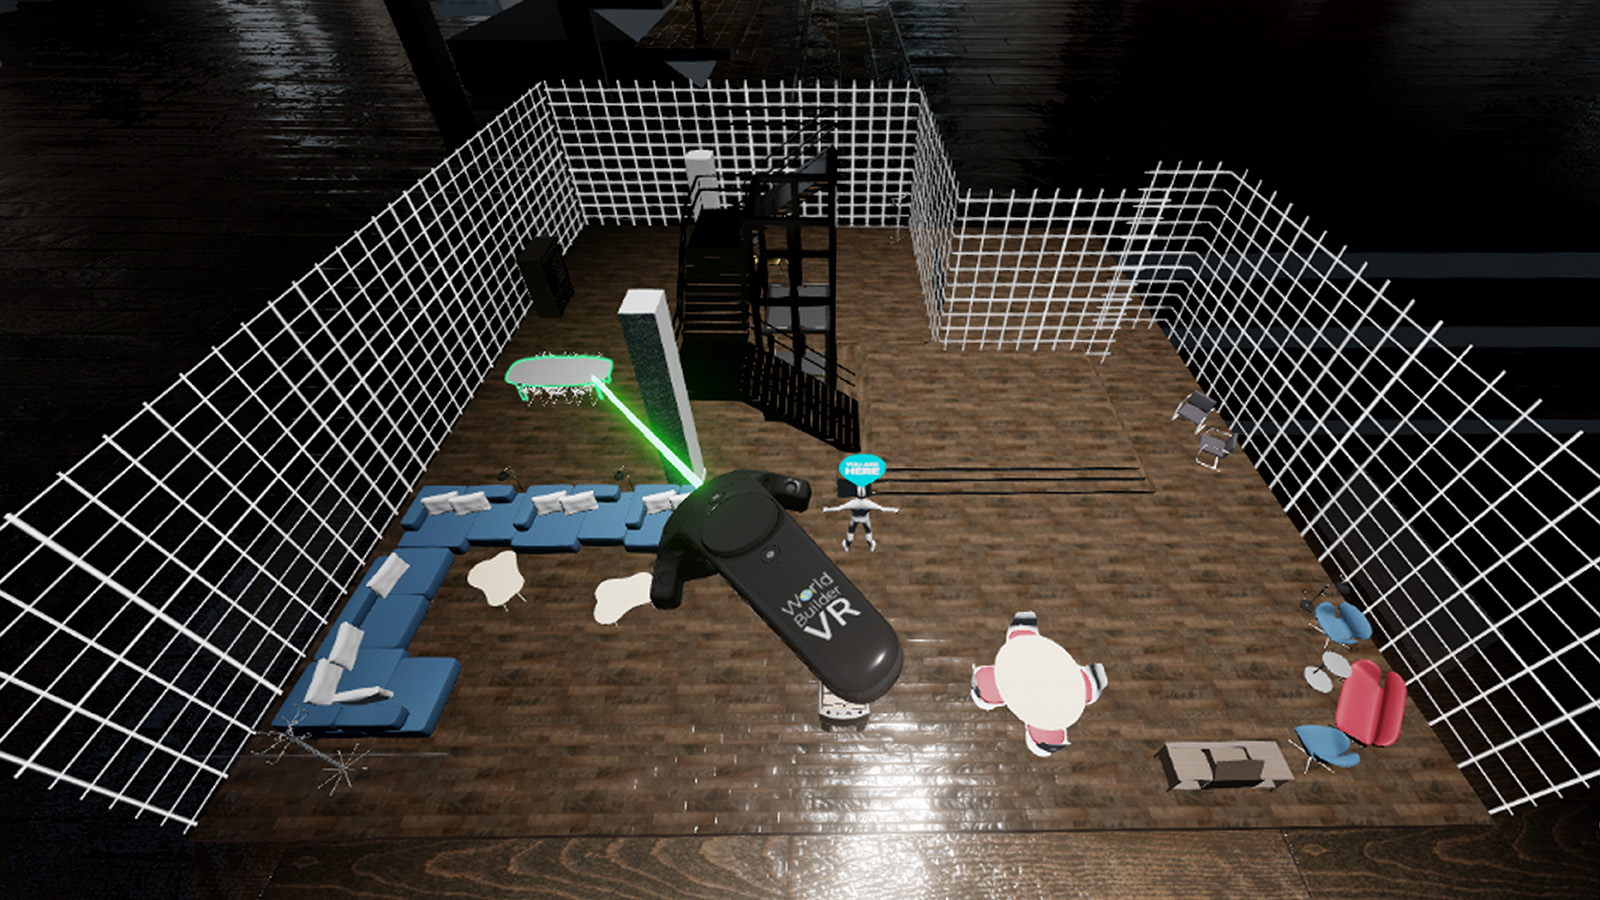
\includegraphics[width=14cm]{kapitel/mini-map.jpg}
  \centering
  \caption{Mini map as part of the WIM technique. By \cite{Arnowitz.2017}}
  \label{fig:minimap}
\end{figure}
An alternative to this method is the world in miniature (WIM) technique. As seen in figure \ref{fig:minimap}, the user gets a miniature map of the virtual world with all selectable objects. The user can now select the desired object in the map and it gets highlighted in the virtual world. With this method, the user looses their ego centred point of view. This can be seen as a decrease in an immerse experience, although it increases usability.

When it comes to moving in the virtual world, the problem of only seeing the virtual world but not the physical world becomes more real. There is a danger of physical damage when colliding with real world object while wearing a HMD. There is a conflict between the real world limited space and the unlimited virtual world (TODO source). Therefore some techniques are described also by \cite{Dorner.2013} how to deal with the problems of navigating through virtual worlds:\\
One method of moving around in VR can be the direct manipulation of the camera with a suitable input controller. The user moves the camera with the help of a joystick for example. Another method, which is very common in 3D computer games and therefore conforms highly to the expectations of users, is the walking in the direction of the user's point of view. A disadvantage of this method is, that the user cannot look around while moving. Both described techniques have the disadvantage, that they can cause motion sickness. This phenomenon will be described in chapter \ref{limits}.\\
To overcome the motion sickness problem, a very common technique for navigation is teleporting. Teleporting means to translate the user directly to a specific position without a time delay. The technique can be realised in VR by selecting the desired translation point via ray-casting and jumping to the point after selection. This method successfully overcomes the problem of motion sickness, but there is a loss of immersion, since this kind of navigation is not very natural.  \cite{Bozgeyikli.2016}\\
The most natural and immerse way of navigating is physical walking. Walking in a virtual environment deals with all the problems of space and the above mentioned conflict between real and virtual world space. Natural walking in general needs more complex hardware for tracking the users movement than navigation with the help of a hand controller. One method of walking in VR is the walking in place method. As the name describes it, the user moves in the virtual world by lifting their legs but they are not actually changing their position in the real world. There are several hardware installations which support walking in place, some of them make walking possible through a treadmill like system.\\
It is also possible to let the user walk around in room which was designed for virtual reality usage and provides suitable tracking sensors. To avoid colliding with the real world borders of the room, the redirected walking technique was developed. With this technique it is possible to make the user believe they are walking straight, while small changes in the virtual world make them actually move in circles or in similar paths as seen in figure \ref{fig:walking}
\begin{figure}[h!]
  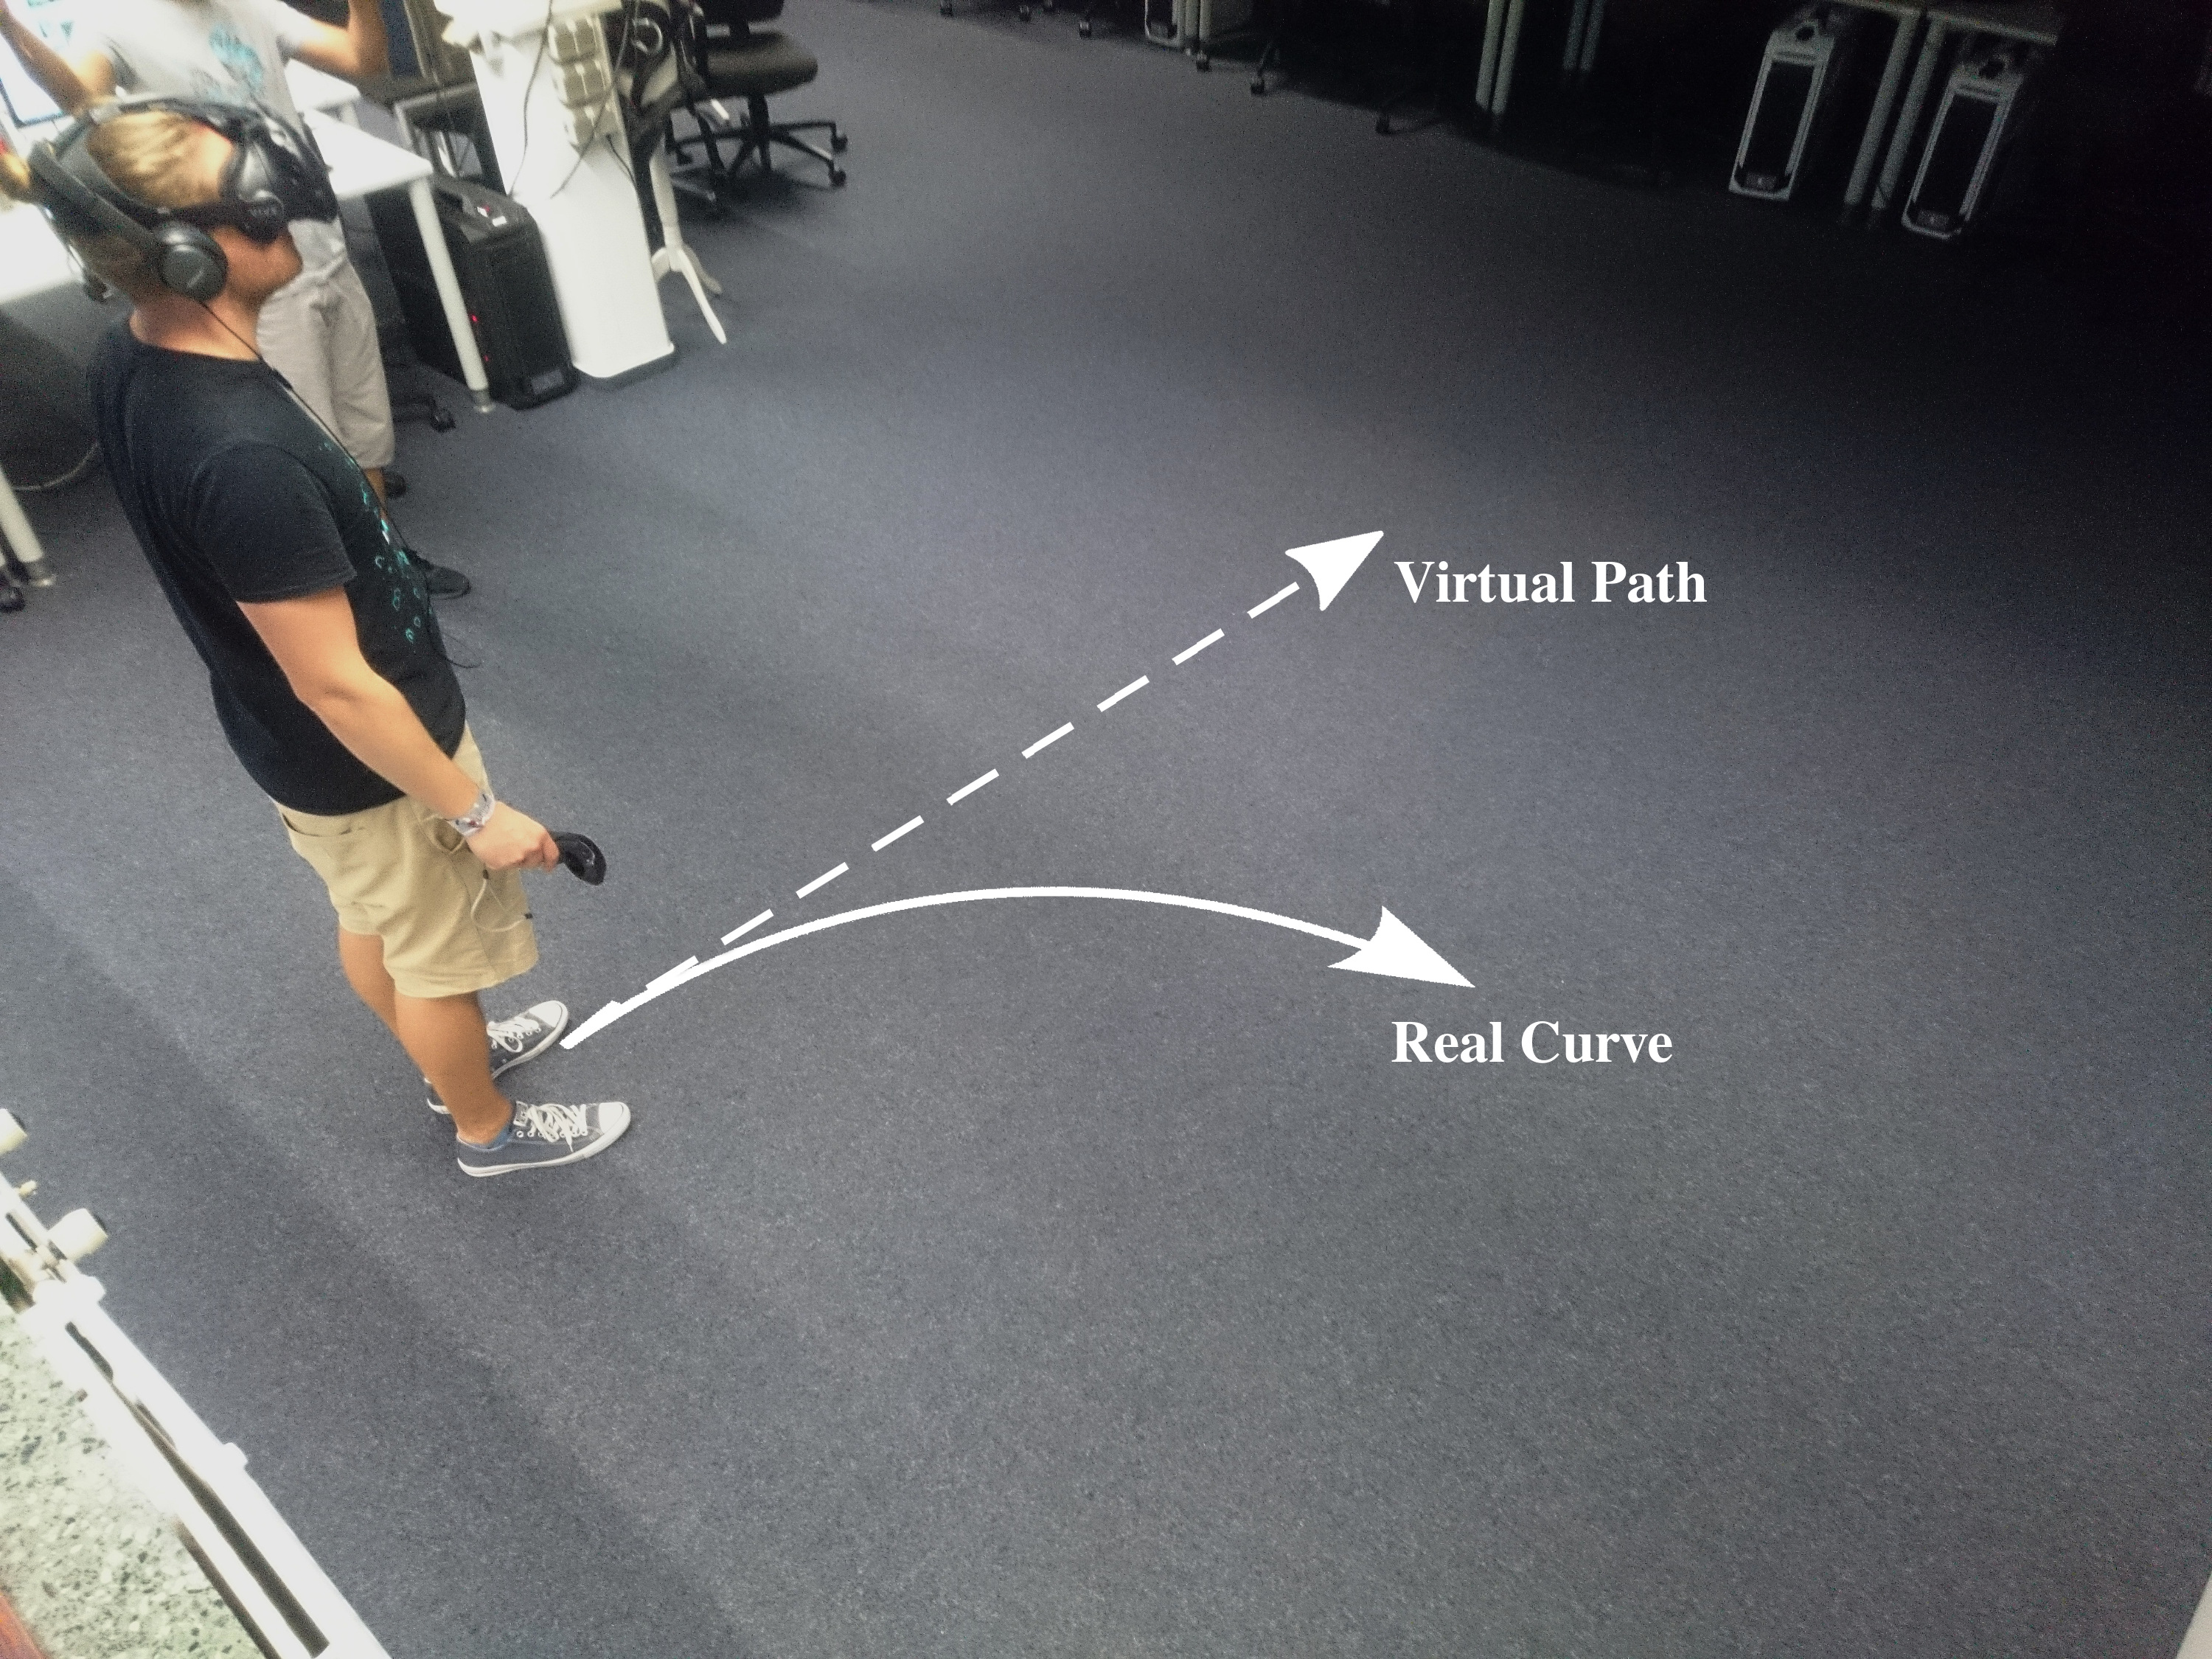
\includegraphics[width=10cm]{kapitel/redirected-walking.jpg}
  \centering
  \caption{Redirected walking in VR, virtual walking path vs. actual walking path. By \cite{LS18}}
  \label{fig:walking}
\end{figure}

\section{Hardware for VR}
\todo{describe difference between mobile and desktop HMDs, show examples HTC Vive and Google Daydream, maybe also Google Cardboard. What possibilities of interaction do they provide?}
There has been a lot of research in hardware technologies to support physical immersion in VR. Some important objectives when it comes to new hardware technologies in VR are the increase of immersion, the reducing of costs and the decreasing of size and weight. The two main types of HMDs currently available are the desktop HMDs and the mobile HMDs. The first type runs the application on a standalone desktop and the HMD measures the sensorical data from the user. The second type uses the phone to run the application and the phone's sensors to measure head rotation and other relevant data. For the application of this project, the Samsung Gear VR headset is used, which is a mobile HMD. In order to understand the advantages and disadvantages of mobile phone based HMDs, it is compared to the desktop pc based HMD HTC Vive pro. This chapter will compare the HMDs in the aspects of usability, ammount of immersion and price classes. Both devices can be seen in figure \ref{fig:devices}.

\begin{figure}[h!]
  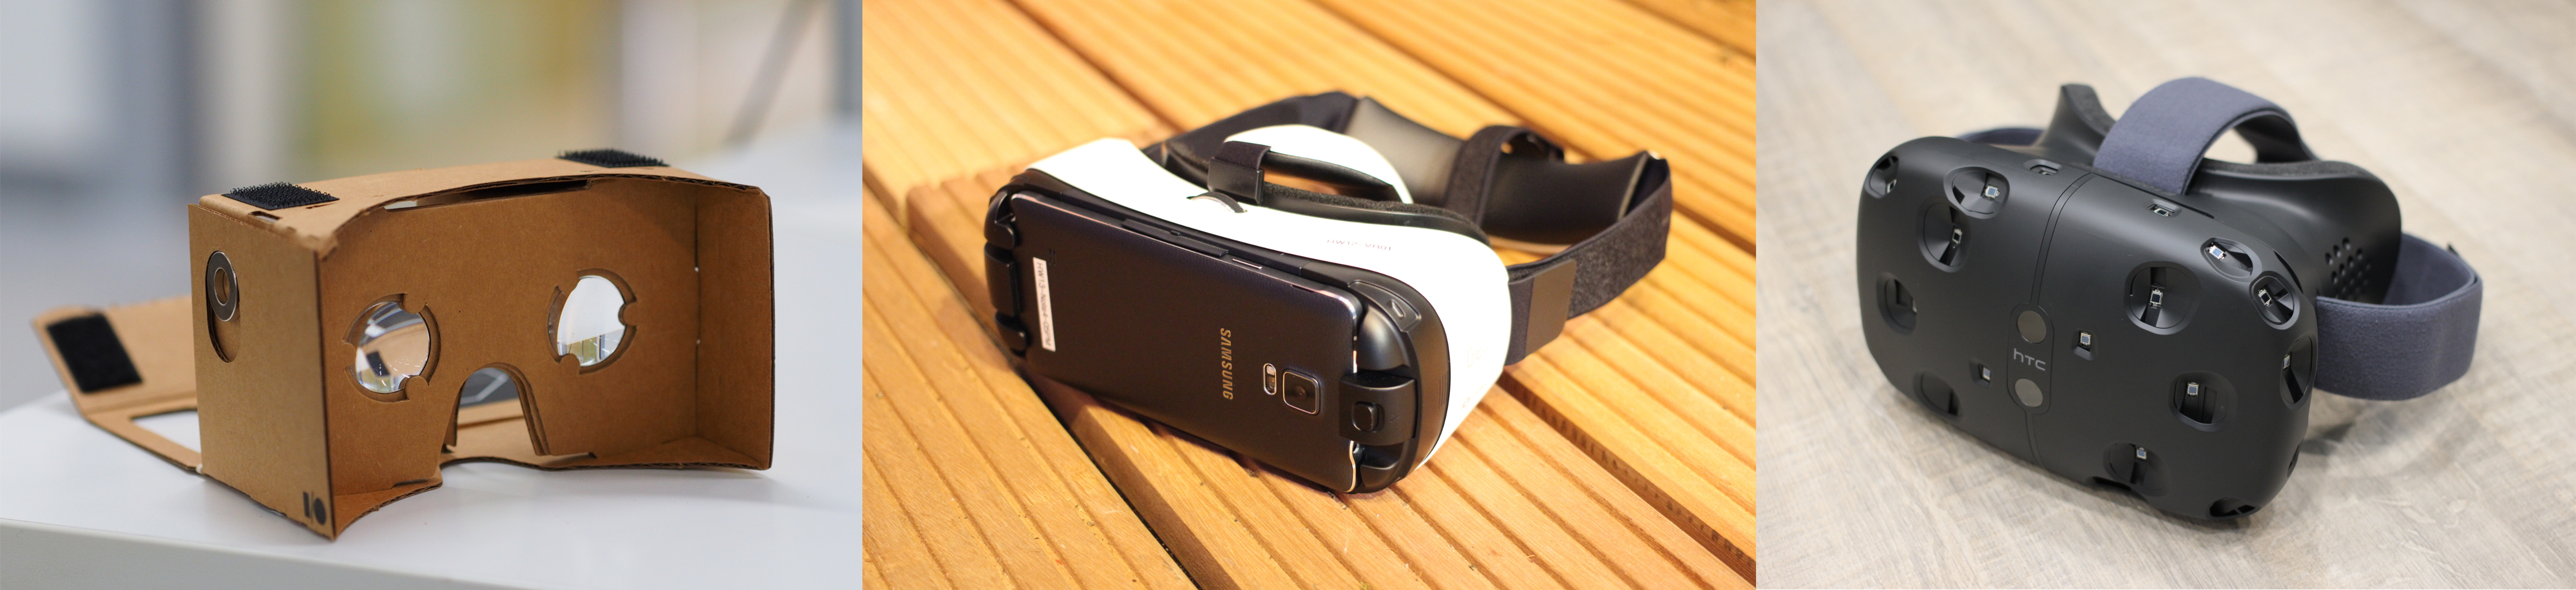
\includegraphics[width=14cm]{kapitel/hmd-devices.jpg}
  \centering
  \caption{From left to right: Google cardboard \cite{cardboard}, Samsung Gear VR \cite{gearvr}, HTC Vive \cite{vive}}
  \label{fig:devices}
\end{figure}

\paragraph{Google cardboard}
Google cardboard is a HMD introduced in 2014. It is a mobile VR headset, which means that the VR application is running on a mobile device embedded in Google cardboard's case (see fig TODO). Google cardboard uses the sensors (gyroscope, accelerometer, etc.) of the phone, the phone's screen, splitted into two views for each eye to display the content and lenses for the viewing. All components are held together by a case made of cardboard The special feature of Google cardboard are the low costs. When introduced, Google published the cutting template for the case for free (TODO source). The objective of Google cardboard was to arise interest in VR to a more widespreaded audience by reducing the costs and accesability to a minimum. There are a variety of applications supporting Google cardboard on playstore, most of them available for free. \cite{Tham.2018} \\
The disadvantages of Google cardboard are that the hardware is limited to the capacity of the phone which results in low screen resolution and limited performance.
In 2016 Google has anncounced the successor of cardboard, the Google Daydream VR. This device has more advantage HMD case and input controllers \cite{??}.

\paragraph{Samsung Gear VR} Samsung Gear VR is a mobile based VR headset which was developed by Samsung and Occulus, introduced in 2017. Similar to Google cardboard, the performance and screen resolution of the HMD depends on the mobile phone, used with the headset. Gear VR is currently supported only by the newer Samsung phones, including Galaxy S6 and higher, Galaxy Note 5 and higher, Galaxy A8 and higher.
It comes with a bluetooth hand-held controller which can either be held in the left or right hand. Inside the HMD is a gyro sensor to detect algignment and orientation of the device. There is a proximity sensor as well in the headset to detect if the user is currently wearing the HMD.  \cite{Samsung.2019}\\
The price of the Gear VR is currently 130 USD, which is more expensive than the Google cardboard or daydream, but cheaper than the desktop based HMDs available on the market at the time of writing. (TODO source)\\
The Gear VR works intuitive with the supported devices and is supported by the game engine unity, which makes the software application development easier. However, the use of a Samsung mobile phone is required, and not all Samsung phones are supported.
\paragraph{HTC Vive Pro}
The HTC Vive pro is a VR headset which was released in April 2018. It provides a high screen resolution, currently 2550 x 1600 pixels, higher than mobile based HMDs can achieve. The HTC Vive pro has to be connected to a standalone computer station via a cable, a wireless version is under development. The headset comes with two handled controllers and two base stations, which are infrared sensors. 
These two base stations mark a play area, which can be the size of a room or smaller sizes for VR applications played while standing or sitting. Only user interactions done within the play area are recognised by the system. \cite{Ogdon.2019}
The advantages of th HTC Vive Pro are the high performance, high screen resolution and better physical immersion, the disadvantages the high costs (TODO search price) and the need of space because of the play area.

\section{Showcases of VR applications}
There are a variety of VR applications available for very different use cases and made with diverse concepts. The following chapter will present one VR application which is of the category of 360 degree videos, one application from the field of gaming and the last application will be about education and learning.
\section{Limits of VR} \label{limits}
\todo{At current status, what is VR not able to achieve? What are the challenges VR researchers face currently?}
The idea of VR is not a new invention of the past few years. There has already been a peek in research and also prominence to the public in the late 90's and beginning of 2000. However, the technology did not prevail in the economy, because there were several limitations especially in performance of computation. Therefore only a limited amount of ideas were able to be actually implemented. Another problem at that time were the very large and heavy HMDs (TODO insert image). The user could not wear them for a very long time and it caused neck pain and other physical problems. The devices were also not portable. \cite{Jerald.2016}\\
Looking at VR technologies now, a lot has changed. At first, the performace of our processors have increased rapidly. Secondly the HMDs became a lot smaller and lighter compared to the ones of the late 90's. But yet, we are not at the point, where all research is done -- on the contrary: A lot of challenges still occur when creating a VR application today. In the following, the problem of motion sickness will be explained. It will also be pointed out, what solutions are upcoming in the near future. There is also a lot of research in progress, when it comes to maximise physical immersion. It will be explained, what interactions cannot be covered by today's hardware, and what technologies are in development or testing at current stage.
\subsection{Motion sickness}
Motion sickness is a very common problem in VR. It can be compared to the kind of sickness, some people experience when being in moving vehicles, such as buses, cars or roller coasters. The symptoms are nausea, dizziness or even vomit. Most of the time this symptoms occur after a usage time of more than 10 minutes. Unfortunately, motion sickness does not occur on a very small percentage of people and therefore cannot be ignored easily. In the study of \cite{Siess.2017}, over a half of the test persons experienced one of the described symptoms during playing a VR roller coaster game.\\
The most likely reason for motion sickness in VR is the mapping between real movement and virtual movement. For example, there is a high propability of feeling sick, when there is a latency between head movement and the movement in the virtual world. This latency  will be registered by the brain and is experienced as unfamiliar and weird. Other situations, such as walking in the virtual world without physically moving can be a reason for motion sickness as well. \cite{Dorner.2013} \\ \cite{Siess.2017} also listed other reasons such as excessive speeds, for example first person moving speed or the moving speed of nearby obstacles, insufficient graphics or general technical problems( e.g. quality of lenses or comfort of HMD).
\cite{Fenlon.2013} mentions the removal of player control as a reason for motion sickness. It is more likely to experience the symptoms, if the games takes control over the head rotation instead of the player. \\
To overcome the problem of motion sickness, the latency between physical and virtual movement has to be as small as possible. This is of course limited by the performance of the hardware devices. Many creators try to manage the problem by creating short time experiences with less than 10 minutes durance and trying to avoid fast moving objects in their application. \cite{Doerner.2013}\\
This approach however, limits the possibilities of VR applications. It would be hard to create an action shooter without fast moving objects, for example. \\
Besides this constraints, there have been new hardware developments lately, which promise to solve the problem of motion sickness in VR. One of this hardware inventions is a device by \cite{?} with vibration motors attached to it. User wear a headband with the motors placed near to the ear. Everytime users move in the virtual world, the vibration motors provide a haptic feedback. According to \cite{?} this vibration should affect the vestibular system and deludes a movement to the brain. The gap between physical and virtual movement can be tricked in a way through the device. However, the headband is still a prototype and so far, the effects and reasons for it are a hypothesis. There have to be more clinical studies until a clear statement of the effectiveness can be made.\\
Looking at the VR prototype application, which will be developed during this work, the risk of motion sickness should be held to a minimum. To fulfill this requirement, a balance between a high level of immersion and the reducing of motion sickness has to be hold. How this is realized, will be described in chapter \ref{design} and \ref{implementaion}. If the requirement is fulfilled, will be reviewed in chapter \ref{testing}.

\subsection{Hardware}
There are several limitations in hardware devices when it comes to VR at the time of writing. First of all, the sensors of a HMD have to work very accurate. Also computation of the head movement and the virtual world movement has to be as fast as possible (see previous chapter). The display resolution is too low currently. Screen resolutions which are working well when it comes to desktop screens or mobile screens do not work so good in VR, because the lenses zoom the picture and the pixels become visible. \\
When looking at physical immersion, there are a lot of potential enhancements in providing the user a more natural way of interacting with the virtual world. Hand held controllers have to be used in with  the most commercial available HMDs. A body tracking system would provide more immersion, but requires very accurate sensors.
Relocating the player in the virtual world is also a challenge at the time of writing. In chapter ?? the use of treadmill system was already mentioned. The following section will present a current available VR treadmill for VR. Within this example the current limits of physical walking VR are explained.

In \cite{Cakmak.2014} the cyberith virtualizer is introduced. It is a device which supports natural walking in VR through the walking in place method. Users are wearing special shoes and lean into a belt system, which can be seen in figure TODO. The feet are sliding onto the surface and translated as a movement into the virtual world. The movement mapping is realized through various sensors which are placed into the ground floor of the treadmill. It is possible to use the cyberith virtualizer with controller specialized games, because the software of this treadmill is emulating controller input commands.\\
This device, however is not yet available on the consumer market. The company had problems of finding customers after announcing and presenting it in 2014. In 2016 they announced that they would concentrate on the B2B market and yet they are not in serial production in 2019. \citep{TODO}\\
The reasons for this could be the expensive price and also the large size of the device. The consumer market might not be ready yet for devices like that. This example shows how challenging it is for commercial companies to make innovations in VR. Therefore it is important to push public scientific research in VR further forward.

\section{Measurement of effectiveness of VR applications}
\todo{name existing questionnaires about immersion, explain why they do not cover all aspects which are required for this application}

